%\section{Contact Graphs and Disk Arrangements}
%% Outline:
%% 1) What is the goal of this section?
%% 	a) What is needed to achieve this goal?
%% 	b) Formally pose the problem.
%% 	c) How is (a) used to solve (b)?
%Using logic engines, it has been shown that it is NP-Hard to decide whether the graph $G$ is a contact graph of unit disks \cite{BET+99}. 
%\begin{thm}\label{thm:ContactGraphV3-1}
%It is NP-complete to decide whether a polygonal linkage whose hinge graph is a tree can be realized.
%\end{thm} 
%\begin{proof}
%proof goes here
%\end{proof}
%We take the proof of Theorem \ref{thm:ContactGraphV3-1} and adapt it to contact graphs, i.e.:
%\begin{thm}\label{thm:ContactGraphV3-2}
%It is NP-complete to decide whether a contact graph can be realized.
%\end{thm}
%In order to show this, we will review some properties about contact graphs.
%\subsection{Contact Graph Properties}
%\paragraph{Hausdorff Distance}  Let $A$ and $B$ be sets in the plane. The \textit{directed Hausdorff distance} is 
%\begin{equation}\label{eqn:ContactGraphV3-1}
%d\lr{A,B} = \sup_{a \in A} \inf_{b \in B} \left\vert\left\vert a-b \right\vert \right\vert
%\end{equation}
%$h\lr{A,B}$ finds the furthest point $a in A$ from any point in $B$.  \textit{Hausdorff distance} is
%\begin{equation}\label{eqn:ContactGraphV3-2}
%D\lr{A,B} = \max \left\lbrace d\lr{A,B}, d\lr{B,A} \right\rbrace
%\end{equation}
%\begin{figure}[!htbp]
%\begin{center}
%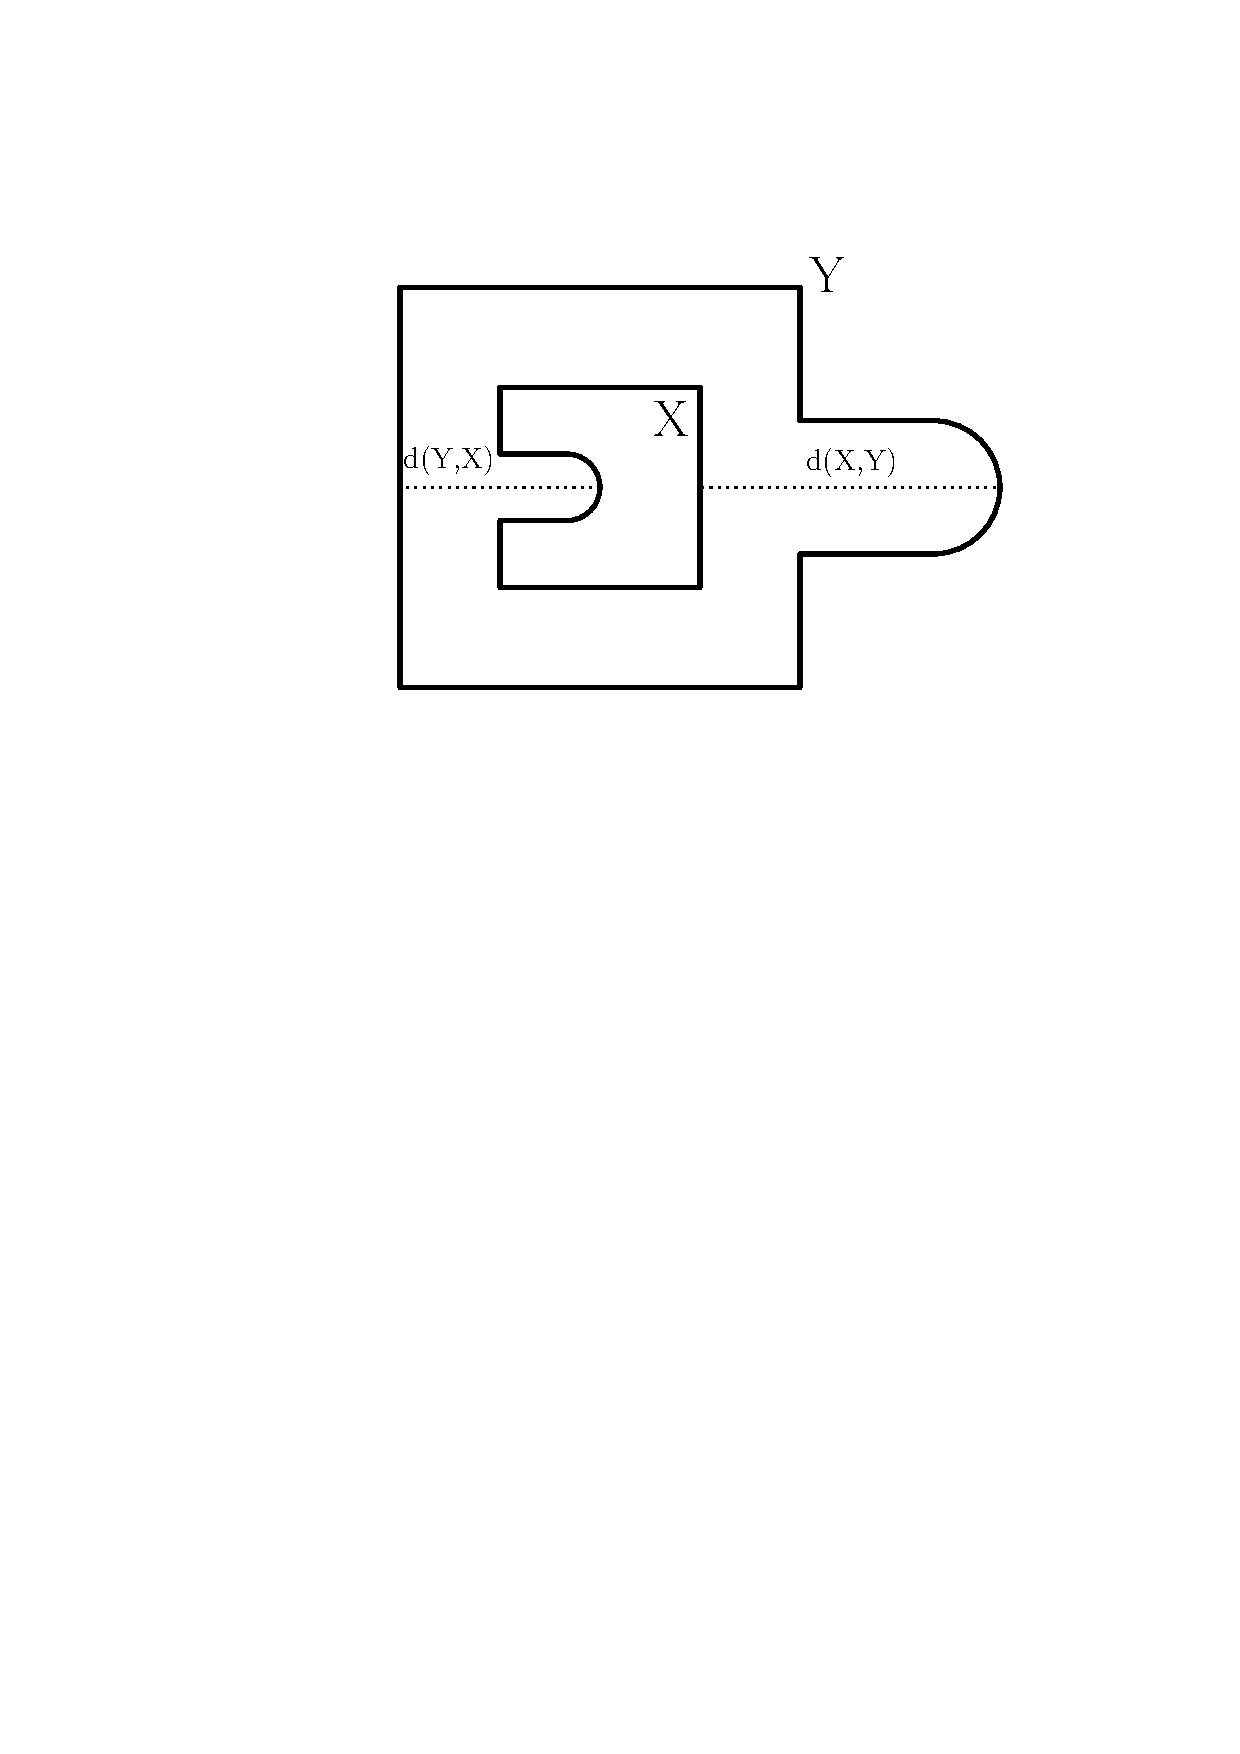
\includegraphics{graphics/HausdorffDistanceExample1.pdf}
%\caption{An illustrative example of $d(X,Y)$ and $d(Y,X)$ where $X$ is the inner curve, and $Y$ is the outer curve.}\label{fig:HausdorffDistanceExample1.pdf}
%\end{center}
%\end{figure}
%\paragraph{$\epsilon$-approximation}
%% Modeling the logic engine with polygonal linkages requires reflected copies of the
%% rectangles. For an oriented realization, we use a different technique in Section 3. The
%% above proof can be adapted to the realization of contact trees of disks by approximating
%% rectangles with disk arrangements. In this context, we say that a weighted graph G is a
%% ε-approximation of a polygon P if G is realizable as a contact graph of disks of given
%% radii, and in every such realization, the Hausdorff distance between the union of disks
%% and a congruent copy of P is at most ε. A weighted graph G is a stable ε-approximation
%% if, in addition, for every two such realizations of G, the distance between the centers of
%% the corresponding disks is at most ε after a suitable rigid transformation.
%The weighted graph, $G$, is an \textit{$\epsilon$-approximation} of a polygon $P$ if the Hausdorff distance between every realization such realization of $G$ as a contact graph of disks and a congruent copy of $P$ is at most epsilon.  A weighted graph $G$ is said to be a \textit{$\BigOh{f(x)}$-approximation} of a polygon P if there is a positive constant $M$ such that for all sufficiently large values of $x$ the Hausdorff distance between every realization such realization of $G$ as a contact graph of disks and a congruent copy of $P$ is at $M \cdot \vert f(x)\vert$. A weighted graph $G$ is said to be a \textit{stable} if it has the property that for every two such realizations of $G$, the distance between the centers of the corresponding disks is at most $\epsilon$ after a suitable rigid transformation.  
%
%
%
%
%
%\begin{lem}\label{lem:ContactGraphV3-1}
%For any natural number $k$,  there exists a tree $T = (V,E)$ with vertex weights $1$ and $1 - k^{-3}$ such that a stable $\BigOh{k^{-1}}$-approximation of a rectangle with ratio $\sqrt{3}$.
%\end{lem}
%\begin{thm}\label{thm:ContactGraphV3-3}
%It is NP Complete to decide whether a given tree with positive vertex weights is the contact graph of a disk arrangements with specified radii.
%%1) needs to show that
%\end{thm}
%
%\begin{figure}[!htbp]
%\begin{center}
%\includegraphics{graphics/snowflakeOutline5Layer}
%\caption{Insert Caption}\label{fig:snowflakeOutline5Layer}
%\end{center}
%\end{figure}
%
%\begin{pf}
%\begin{itemize}
%\item[(i)]  To prove \ref{thm:ContactGraphV3-3}, we need to show the following:
%	\begin{itemize}
%	\item[(a)] blah blah
%	\item[(b)] blah blah
%\end{itemize}
%\item[(ii)] Once we have (i), we then proceed with...
%\end{itemize}
%\end{pf}





%%%COMMENTS FROM MEeting
%Introduction:recall contact tree of disks with radii is hard.  
%tool to prove is approx hexagonal tiling with disks.  Find NP Hardness Reduction via arrangement of hexagons with disks
%modelling the hexagons with the arrangement of disks; r_0 = 1  r_i = 1 + \epsilon
%state it intuitively with examples
%stability: every realization is close to the hexagon graph with weights on vertices.  the disnce between the centers of hexagonal lattice and contact graph are close
%property of a vertex weighted graph if for any two realizations has a \ldots let G be an ordered tree with any two realizations R_1, R_2.  G is \epsilon stable with any two realizations the vertices are close.  there exists a rigid transformation \gamma such that the vertices\left(\gamma\left(R_1 \right)\right) - vertices\left(\gamma\left(R_2\right)\right) < \epsilon
%1) state goal of theorem
%2) state theorem: Hexagon of side length 1, for any \epsilon > 0, there exists an oriented vertex weighted tree that satisfies the following:
%	a) |V| is defined polynomially as a function of epsilon
%	b) all weights are bounded by some polynomial as a function of epsilon
%3) prove step by step:
%	a) define the tree
%	b) show that any realization of the tree is close to T_i, i.e. for any realization of a tree there exists a T_i such that H(T_i,P)<\epsilon
%4) proof by induction
%	a) one for the angles
%	b) one for the centers
%	c) fuzzy hexagons approximate regular hexagons are approximal from the same proof
%Define tree by i^{th} layer
%try defining without realization abstract
%NTS T_{i,\epsilon} there exists a realization R\left(T_{i,\epsilon}\right) hint lattice -> introduce \epsilon  start with

\section{Contact Graphs and Disk Arrangements}



\begin{figure}[!htbp]
\begin{center}
\includegraphics{graphics/snowflakeOutline5LayerSmall.pdf}
\caption{A configuration of disks about a snowflake.}\label{fig:snowflakeOutline5Layer}
\end{center}
\end{figure}

\begin{thm}\label{thm:ContactGraphV3-1}
It is NP-complete to decide whether a polygonal linkage whose hinge graph is a tree can be realized.
\end{thm} 